% ----------------------------------------------------
% Literature Review
% ----------------------------------------------------
\documentclass[class=report,11pt,crop=false]{standalone}
% Page geometry
\usepackage[a4paper,margin=20mm,top=25mm,bottom=25mm]{geometry}

% Font choice
\usepackage{lmodern}

% Wrap text around image
\usepackage{wrapfig}

% Checkmarks
\usepackage{tikz}

% For algorithms
\usepackage[]{algorithm}
% Pseudocode packages
\usepackage{algpseudocode}

% Table color
% \usepackage{colortbl}

% Multiple rows
\usepackage{multirow}

% Lorem ipsum
\usepackage{lipsum}

% Use IEEE bibliography style
\bibliographystyle{IEEEtran}

% Line spacing
\usepackage{setspace}
\setstretch{1.20}

% Ensure UTF8 encoding
\usepackage[utf8]{inputenc}

% Language standard (not too important)
\usepackage[english]{babel}

% Skip a line in between paragraphs
\usepackage{parskip}

% For the creation of dummy text
\usepackage{blindtext}

% Math
\usepackage{amsmath}

% Lists
\usepackage{enumitem}

% Header & Footer stuff
\usepackage{fancyhdr}
\pagestyle{fancy}
\fancyhead{}
\fancyhead[R]{\nouppercase{\rightmark}}
\fancyfoot{}
\fancyfoot[C]{\thepage}
\renewcommand{\headrulewidth}{0.0pt}
\renewcommand{\footrulewidth}{0.0pt}
\setlength{\headheight}{13.6pt}

% Epigraphs
\usepackage{epigraph}
\setlength\epigraphrule{0pt}
\setlength{\epigraphwidth}{0.65\textwidth}

% Colour
\usepackage{color}
%\usepackage[usenames,dvipsnames]{xcolor}

% Hyperlinks & References
\usepackage{hyperref}
\definecolor{linkColour}{RGB}{77,71,179}
\hypersetup{
    colorlinks=true,
    linkcolor=linkColour,
    filecolor=linkColour,
    urlcolor=linkColour,
    citecolor=linkColour,
}
\urlstyle{same}

% Automatically correct front-side quotes
\usepackage[autostyle=false, style=ukenglish]{csquotes}
\MakeOuterQuote{"}

% Graphics
\usepackage{graphicx}
\graphicspath{{Images/}{../Images/}}
\usepackage{makecell}
\usepackage{transparent}

% SI units
\usepackage{siunitx}

% Microtype goodness
\usepackage{microtype}

% Listings
\usepackage[T1]{fontenc}
\usepackage{listings}
\usepackage[scaled=0.8]{DejaVuSansMono}

% Custom colours for listings
\definecolor{backgroundColour}{RGB}{250,250,250}
\definecolor{commentColour}{RGB}{73, 175, 102}
\definecolor{identifierColour}{RGB}{196, 19, 66}
\definecolor{stringColour}{RGB}{252, 156, 30}
\definecolor{keywordColour}{RGB}{50, 38, 224}
\definecolor{lineNumbersColour}{RGB}{127,127,127}
\lstset{
  language=Matlab,
  captionpos=b,
  aboveskip=15pt,belowskip=10pt,
  backgroundcolor=\color{backgroundColour},
  basicstyle=\ttfamily,%\footnotesize,        % the size of the fonts that are used for the code
  breakatwhitespace=false,         % sets if automatic breaks should only happen at whitespace
  breaklines=true,                 % sets automatic line breaking
  postbreak=\mbox{\textcolor{red}{$\hookrightarrow$}\space},
  commentstyle=\color{commentColour},    % comment style
  identifierstyle=\color{identifierColour},
  stringstyle=\color{stringColour},
   keywordstyle=\color{keywordColour},       % keyword style
  %escapeinside={\%*}{*)},          % if you want to add LaTeX within your code
  extendedchars=true,              % lets you use non-ASCII characters; for 8-bits encodings only, does not work with UTF-8
  frame=single,	                   % adds a frame around the code
  keepspaces=true,                 % keeps spaces in text, useful for keeping indentation of code (possibly needs columns=flexible)
  morekeywords={*,...},            % if you want to add more keywords to the set
  numbers=left,                    % where to put the line-numbers; possible values are (none, left, right)
  numbersep=5pt,                   % how far the line-numbers are from the code
  numberstyle=\tiny\color{lineNumbersColour}, % the style that is used for the line-numbers
  rulecolor=\color{black},         % if not set, the frame-color may be changed on line-breaks within not-black text (e.g. comments (green here))
  showspaces=false,                % show spaces everywhere adding particular underscores; it overrides 'showstringspaces'
  showstringspaces=false,          % underline spaces within strings only
  showtabs=false,                  % show tabs within strings adding particular underscores
  stepnumber=1,                    % the step between two line-numbers. If it's 1, each line will be numbered
  tabsize=2,	                   % sets default tabsize to 2 spaces
  %title=\lstname                   % show the filename of files included with \lstinputlisting; also try caption instead of title
}

% Caption stuff
\usepackage[hypcap=true, justification=centering]{caption}
\usepackage{subcaption}

% Glossary package
% \usepackage[acronym]{glossaries}
\usepackage{glossaries-extra}
\setabbreviationstyle[acronym]{long-short}

% For Proofs & Theorems
\usepackage{amsthm}

% Maths symbols
\usepackage{amssymb}
\usepackage{mathrsfs}
\usepackage{mathtools}

% For algorithms
%\usepackage[]{algorithm2e}

% Spacing stuff
\setlength{\abovecaptionskip}{5pt plus 3pt minus 2pt}
\setlength{\belowcaptionskip}{5pt plus 3pt minus 2pt}
\setlength{\textfloatsep}{10pt plus 3pt minus 2pt}
\setlength{\intextsep}{15pt plus 3pt minus 2pt}

% For aligning footnotes at bottom of page, instead of hugging text
\usepackage[bottom]{footmisc}

% Add LoF, Bib, etc. to ToC
\usepackage[nottoc]{tocbibind}

% SI
\usepackage{siunitx}

% For removing some whitespace in Chapter headings etc
\usepackage{etoolbox}
\makeatletter
\patchcmd{\@makechapterhead}{\vspace*{50\p@}}{\vspace*{-10pt}}{}{}%
\patchcmd{\@makeschapterhead}{\vspace*{50\p@}}{\vspace*{-10pt}}{}{}%
\makeatother
\makenoidxglossaries

\newacronym{radar}{RADAR}{Radio Detection and Ranging}
\begin{document}
\ifstandalone
\tableofcontents
\fi
% ----------------------------------------------------
\chapter{Literature Review \label{ch:literature}}
\vspace{0.25cm}
% ----------------------------------------------------
The aim of this chapter is to conceptualize the operation of spectrum analyzers and establish a theoretical foundation for the frequency analysis techniques applied to produce the correct output. This conceptualization is then integrated with a broader review of digitizing and modernizing the display of spectrum analyzers.

In circumventing design limitations of spectrum analyzer displays, it is prudent to survey the most suitable hardware components. This is particularly true for the case where electronic components are required to perform in a broad frequency bandwidth. For example, for high frequency signals, the Nyquist theorem indicates that the ADC is required to have a sample at a frequency that is more than double the frequency of the output signal. Furthermore, the challenge of presenting signals in the frequency domain using electronics exists due to the fact the input signal to the ADC holds information about frequency in the time domain. Therefore, the investigation of literature that is presented in this chapter aims to provide a motivation for the design decisions taken in digitizing and modernizing the HP141T display.

The chapter begins with an evaluation of the frequency domain analysis theory that is applied in the operation of signal analyzers. Then, the different principles that distinguish different types of analyzers are explored to form the basis understanding the expected behaviour of a spectrum analyzer with specific settings. Following descriptions of the operation of spectrum analyzers from literature, the chapter includes a review of the investigation into different techniques for digitizing analyzer displays. This also includes a review of the different electronic components and techniques for digitizing frequency information in order to survey available hardware options that can be selected for a cost effective implementation. Finally, a broad discussion is included on different types of displays for analyzers in literature and a critique of the literature is provided to outline the purpose of the proposed design. 

\section{History and Fundamentals of Spectrum Analysis}

\subsection{Introduction to Spectrum Analysis}

A spectrum analyzers \acrshort{sa}s is a critical instrument for investigating properties of physical phenomena that can be interpreted through power and frequency characteristics of analog signals derived from voltage measurements. This project differentiates between spectrum analyzers and oscilloscopes such that spectrum analyzers are instruments that display waveforms in the frequency domain and oscilloscopes as instruments that operate in the time domain. However, the paper recognizes their significance in signal processing applications, as well as some of the shared similarities in their subsystems. 

As such, the following section is a review of the history and applications of spectrum analyzers and oscilloscopes to establish the context of the project. By assimilating literature on the applications of these instruments in engineering, the section also aims to formulate design guidelines from previous works that can improve the operation of the digitized HP141T, thereby satisfying user and functional requirements. 

\subsection{Early Developments in Waveform Analysis}

The evolution of \acrshort{sa}s is closely linked to that of the oscilloscope. In a review of the history and technology of oscilloscopes, Pereira attributed the invention of the electromagnetic oscillograph to the French physicist, Andr\'{e}-Eugene Blondel \cite{pereira2006}. Oscillographs were devices that used a pen attached to a moving coil to trace an ink record on a rotating paper chart \cite{pereira2006}. According to Herres, the motivation for the invention of oscillographs was to extract waveforms from acoustic and electrical phenomena, however, the devices had a severely limited frequency response and bandwidth because of the inertia of the pen and ink recording equipment \cite{herres2020}. Ultimately, the operation of these devices was restricted by the working principle based on mechanical devices which limited the bandwidth in the range of $10$-$\SI{19}{\hertz}$ \cite{pereira2006}.

\begin{wrapfigure}{r}{0.5\textwidth}
	\centering
	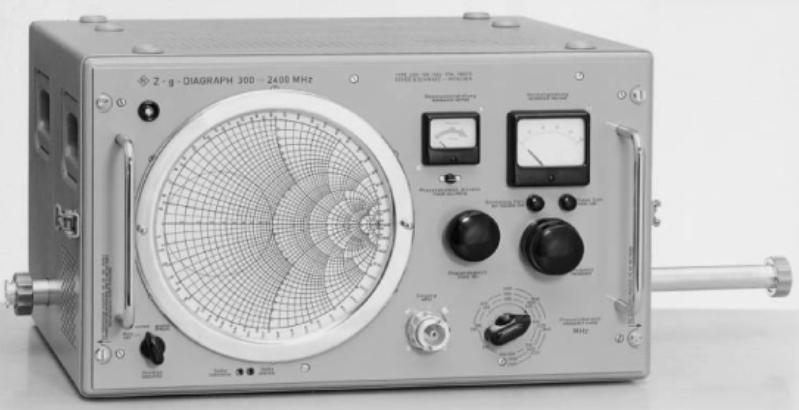
\includegraphics[width=0.50\textwidth]{Figures/Literature_Review/zg-diagraph}
	\caption{The Z-G Diagraph by developed by Rohde \& Schwarz with a Schmidt chart for measuring complex parameters \cite{rytting2008arftg}.}
	\label{fig:zg-diagraph}
\end{wrapfigure}

Following the invention of the oscillograph, available waveform analysis tools included contact diode and vacuum tubes as the only form of signal detectors \cite{vollinger2023}. Technologies such as the slotted line and phase bridges became the standard instruments for measuring amplitude and frequency but were often slow and tedious \cite{rytting2008arftg}. In 1933, Rohde \& Schwarz developed the improved Z-G system which was the first to directly indicate complex parameters on a Schmidt chart as shown in figure \ref{fig:zg-diagraph} \cite{rytting2008arftg}.  

\subsection{Advancements in Spectrum Analysis Technology}
 
The first commercially available real-time signal analyzers (\acrshort{rtsa}s) were introduced in the 1960s by Federal Scientific to process data up to $\SI{20}{\kilo\hertz}$ through a single filter that could change modes in milliseconds \cite{deery2007}. These devices were designed for analyzing mechanical faults and failures in rotating machinery and for investigating vibratory motions of components, systems and structures \cite{deery2007}. In contrast to the the \acrshort{sa}s introduced in the 1960s for characterizing rotary machinery, this paper is focuses on \acrshort{sa}s that were designed for displaying wide-band signals up to the K-band of microwave signals. 

Rapid progress in semiconductor technology and microwave elements laid a foundation for the developed first waveform instrumentation devices with $\SI{1}{\giga\hertz}$ bandwidth \cite{vollinger2023}. With the advent of wireless network technologies, \acrshort{sa} developments became focused on high frequency instrumentation which had to meet testing requirements of first generation technologies such as the \acrfull{amps} operated at frequencies at $\SI{800}{\mega\hertz}$ to $\SI{900}{\mega\hertz}$. Vector network analyzers were introduced as an extension of spectrum analyzers capable of displaying amplitude and phase relative to a reference signal \cite{helfrick2012}. 

\subsection{Early Modifications to Spectrum Analyzers (1960s - 1980s)}

\begin{wrapfigure}{l}{0.6\textwidth}
	\centering
	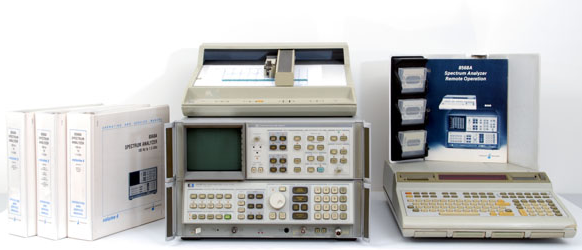
\includegraphics[width=0.60\textwidth]{Figures/Literature_Review/hp8568a}
	\caption{The HP8568A spectrum analyzer which was the first spectrum analyzer from Hewlett-Packard Company to include a microprocessor in the 1970s.}
	\label{fig:hp8568a}
\end{wrapfigure}

Motivated by applications in network analysis and microwave engineering, Hewlett-Packard developed the first fully calibrated spectrum analyzer that capable of sweeping broad frequency ranges \cite{adam1984microwave}. After the introduction of easily-operated wideband network analyzer equipment in 1967, Hewlett-Packard Co. released a network analyzer with a range of $\SI{100}{\kilo\hertz}$ to $\SI{110}{\mega\hertz}$. In particular, the company released the Model 8407A which could resolve amplitude of up to $\SI{0.05}{\decibel}$ on a plug-in polar \acrfull{crt} display to show amplitude and phase \cite{rytandnetwork1969}. The aim of the display was so that the device could be used with Smith chart overlay, or reflection coefficient measurements \cite{rytandnetwork1969}. 

\begin{wrapfigure}{r}{0.40\textwidth}
	\centering
	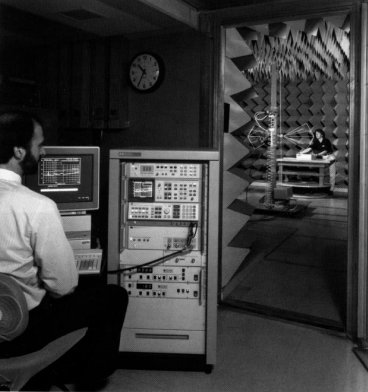
\includegraphics[width=0.40\textwidth]{Figures/Literature_Review/hp8566-large}
	\caption{Illustrating the size of early spectrum analyzer setups. Digitization and modernization of these devices was also focused on reducing their size in order to improve portability.}
	\label{fig:hp56xx-large}
\end{wrapfigure} 

In 1982, D'Addario proposed the implementation of Hewlett-Packard Model 8410A network analyzer as a reflectometer in a system which included an Apple II Plus computer for performing computations of the short-open-load method of calibrating and correcting errors of signals in the S-band of the microwave region of the electromagnetic spectrum \cite{d1982computer}. D'Addario stated that the advantage of implementing a computer-based system was in the software substituted a short delay line for open circuit calibration \cite{d1982computer}. In addition, the software was mostly in Applesoft Basic that featured assembly language subroutines for performing complex arithmetic and controlling the interface \cite{d1982computer}. Similarly, the proposed design in this project aims to exploit the advantages of computerization by introducing functions and libraries for performing digital signal processing tasks and controlling the \acrfull{gui}. 

Another modification to the HP8410 was performed by NASA's Terry and Kunath in 1990, where the \acrshort{sa} was used as an automated far-field antenna range receiver \cite{terry1990}. The system included external mixers capable of harmonic mixing up to $\SI{18}{\giga\hertz}$, \acrfull{adc}s, and interfaced with an external computer \cite{terry1990}. Terry and Kunath noted that the phase and amplitude signals could be converted to digital signals by using either \acrshort{adc}s or by using a digital voltmeter \cite{terry1990}. The authors used a HP308 personal computer with two processors that operated in the DOS 3.3 and HP Basic 5.0 environments, respectively \cite{terry1990}. The computer was employed as the system controller with programs for creating and editing control files for swept frequency, viewing radiated power level data, and running tests with parameters saved in files to be executed or edited at a later time \cite{terry1990}. Consequently, the designer needs to consider file formats, file sizes and file transmission in the process of digitizing a \acrshort{sa}. This is particularly true when the system processes are performed across different devices and programs which may support different file formats and file sizes. 
 
\begin{wrapfigure}{l}{0.6\textwidth}
	\centering
	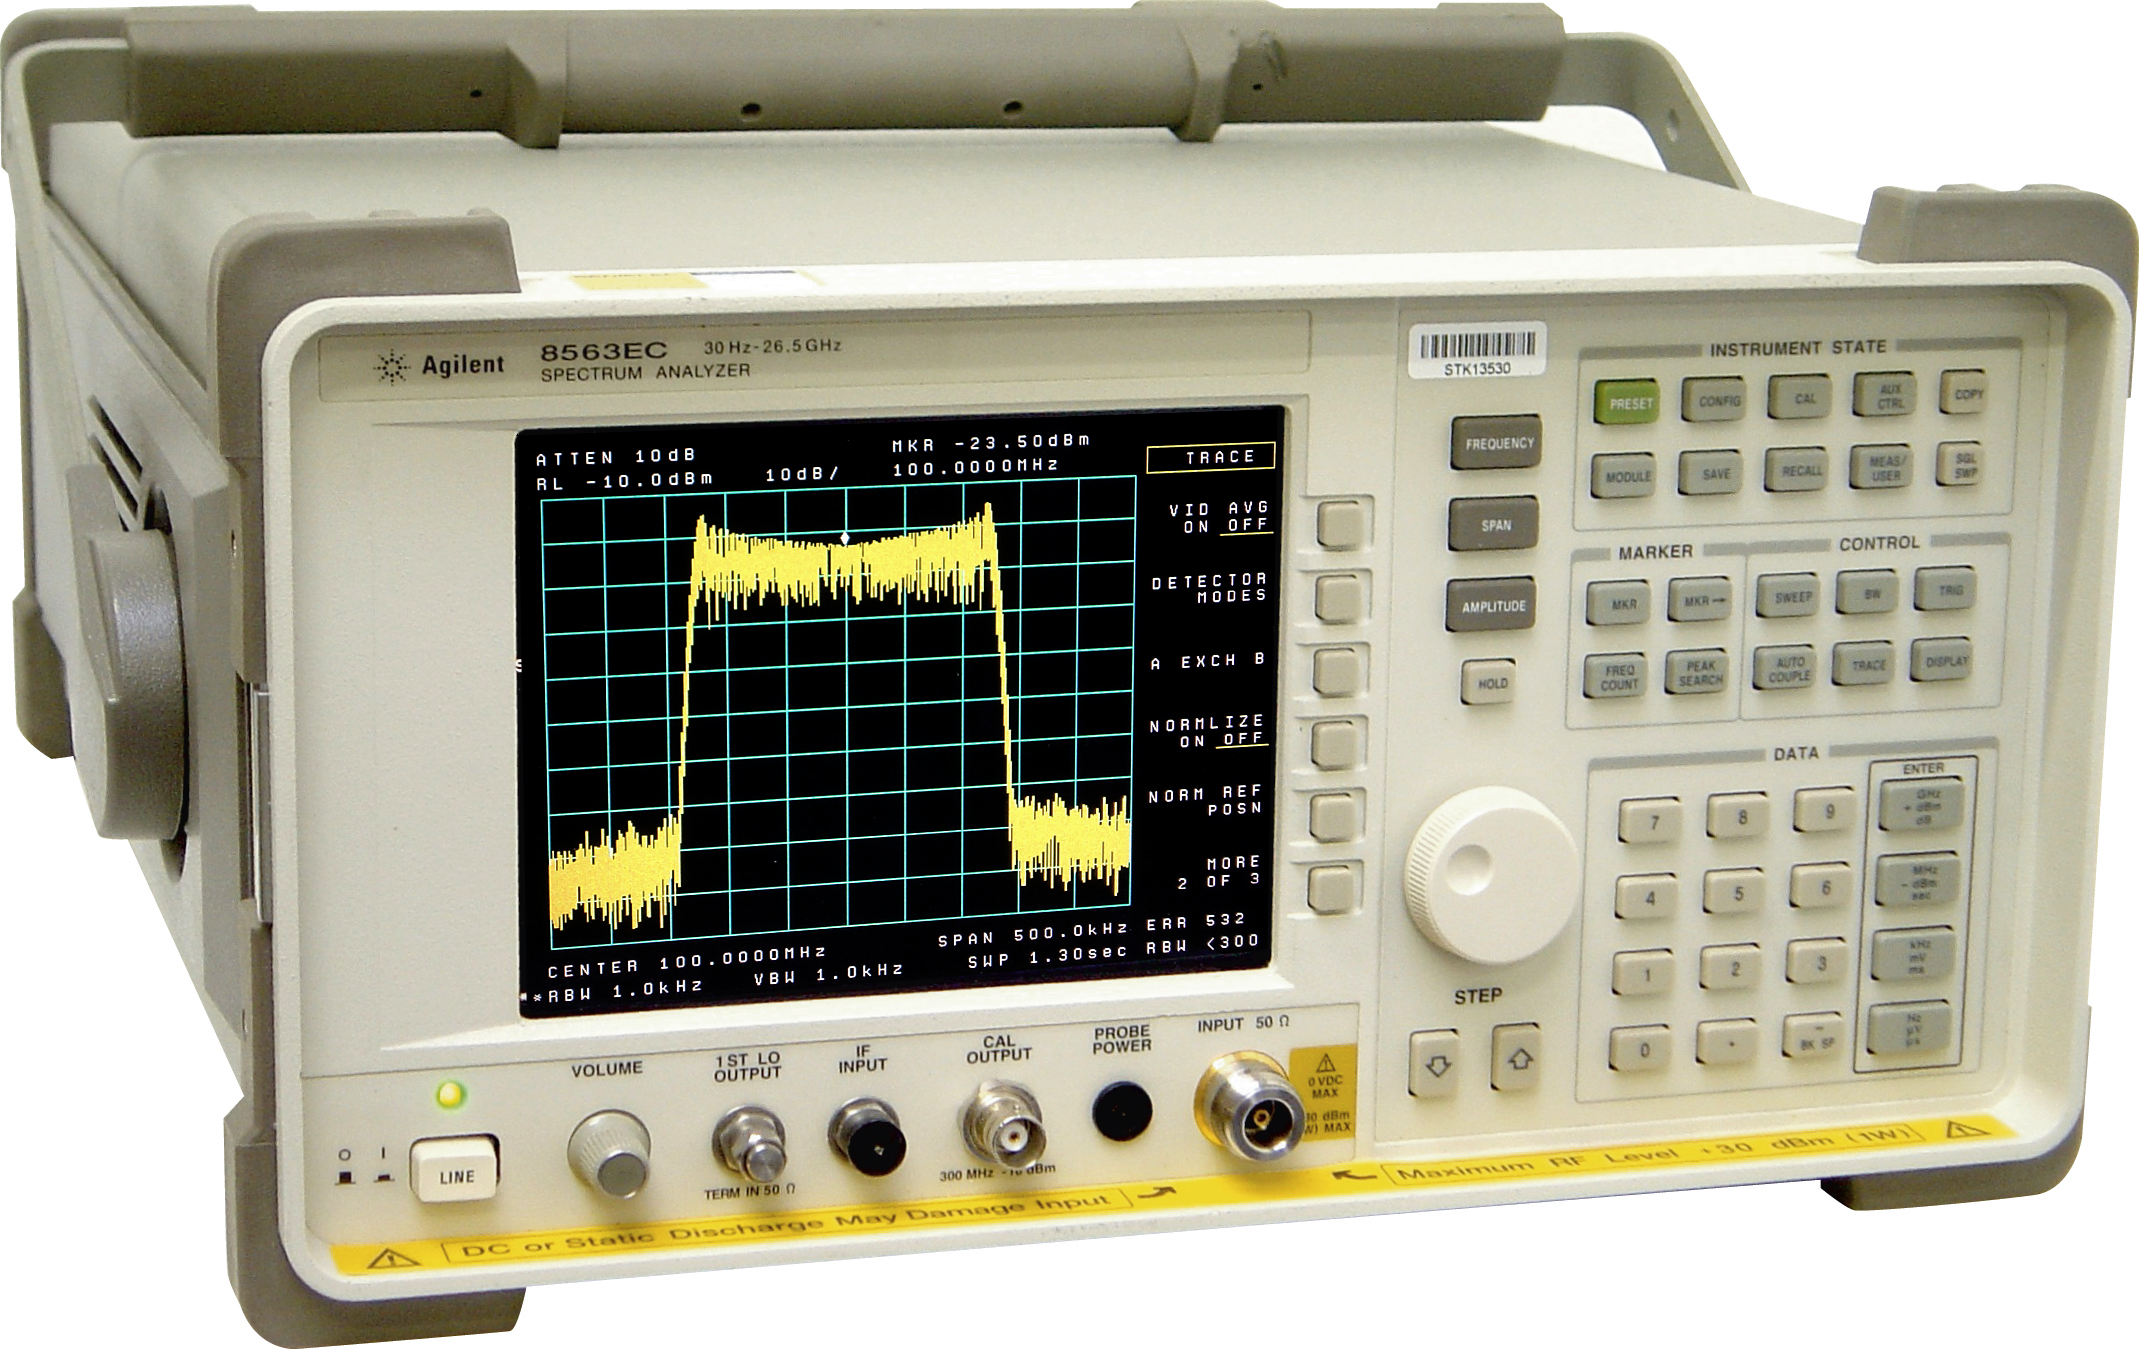
\includegraphics[width=0.40\textwidth]{Figures/Literature_Review/agilent-hp8566EC}
	\caption{The Agilent 8560EC is shown with a \acrshort{lcd} display. This was an improvement over the 8560E model which had a \acrshort{crt} display.}
	\label{fig:agilent-hp8560e}
\end{wrapfigure} 

\subsection{Commercial Digitization of Spectrum Analyzers}

HP85XX spectrum analyzers replaced the HP84XX analyzer series as the first \acrshort{sa}s with synthesized frequency sweeps and an \acrshort{adc} converter for sampling a video signal and displaying it on a \acrshort{crt} screen. The HP85XX series expanded the capabilities of spectrum analyzers, however, earlier versions of these devices were large as shown in figure \ref{fig:hp56xx-large}, where a technician is shown alongside a HP8566B \acrshort{sa} at the heart of two EM1 receivers \cite{hp8566}. Significant improvements to this series of \acrshort{sa}s were realised over previous versions when the HP8568A automatic \acrshort{sa}, shown in figure \ref{fig:hp8568a}, was introduced with a microprocessor controlling its operation. 

In the 2000s, Agilent Technologies mordenized the front and rear panels of HP8560E Model spectrum analyzers,  by introducing \acrshort{lcd} color display interfaced with a \acrshort{lcd} driver board and \acrshort{vga} port located that did not require a user interface \cite{hp8560ec}. Further additions included \acrshort{adc} circuitry integrated into the controller board \cite{hp8560ec}. These improvements also translated into better portability of the system as shown in \ref{fig:agilent-hp8560e}. 

\subsection{Obsolescence and Modernization Strategies}

Overtime as prices of new spectrum analyzers increased rapidly, researchers opted to use older \acrshort{sa}s instead of replacing them. Research into strategies for mitigating risks related to the obsolescence of older \acrshort{sa} models was conducted by Hoppin in 2002, where particular focus was allocated to HP8566/68 \acrshort{sa}s in automated test equipment \cite{hoppin2002}. Hoppin stated that dependence on obsolete and unsupported equipment increased the risk of system and that as \acrshort{sa}s aged, the time required for repair and the cost of replacement increases rapidly \cite{hoppin2002}. As a result of the inevitable obsolescence, Hopping proposed three strategies for dealing with the aged devices, namely, the \textit{stockpile}; the \textit{redesign}; and \textit{migration} strategies. The stockpile strategies requires industry organizations to identify sources of spare replacement components and instruments, and offer repair and calibration services \cite{hoppin2002}. 

This project follows a strategy similar to the redesign strategy proposed by Hoppin in which automated test equipment program managers are required to assess the feasibility of introducing replacement instrument specifications, feature and capability requirements \cite{hoppin2002}. Hoppin noted that one of the risks of applying the redesign strategy is that software projects are notoriously hard to manage to scope, budget and schedule \cite{hoppin2002}. Additionally, since the devices have aged significantly, the languages, tools and methods originally used may be lost, requiring designers to apply reverse engineering techniques \cite{hoppin2002}. To mitigate the costs from applying the redesign process, Hoppin described three main components that need to be considered, namely, test code creation, test instrumentation, purchase and integration, and revalidation measurements and results \cite{hoppin2002}. 

In a similar research published in 2010, Wolle discussed the various aspects related to replacement of obsolete instruments to overcome the challenges that arise when newer versions are not compatible with previous systems \cite{wolle2010}. In the paper, Wolle postulated that an emulation strategy can help designers to incorporate new test instruments to migrate from obsolete instruments \cite{wolle2010}. In addition, Wolle noted that when assessing version migration strategies, modernizing test equipment typically has much higher costs but leads to greater reliability and faster tests \cite{wolle2010}. This was first noted by Hoppin who detailed two risks of implementing a migration strategy as low compatibility and disagreement in measurement results due to differences in architectural and measurement methods between legacy and newer-generation platforms \cite{hoppin2002}.

In a 2014 paper by Iglesias et al., the high cost of spectrum analyzers is also noted as a primary motivation for further developing spectrum analyzer designs \cite{iglesias2014}. Iglesias et al. also indicated that because \acrshort{sa}s employ non-invasive methods to detect machine failures in real-time, the devices need to be continually upgraded to reduce failures by improving the efficiency of industrial monitoring systems \cite{iglesias2014}. Following the motivation for improving \acrshort{sa}s, Iglesias et al. postulated that modernization of \acrshort{sa}s was primarily enabled by the fast evolution of \acrshort{adc}s and \acrfull{dsp}s which offer the opportunity to implement multiple methods for spectrum estimation such as Barlett and Welch's methods for averaging periodograms \cite{iglesias2014}. The authors listed devices such as \acrfull{fpga}s, \acrfull{asic}s, general-purpose \acrshort{cpu}s, and \acrfull{gpu}s as feasible candidates for digitizing \acrshort{sa}s \cite{iglesias2014}, however, \acrshort{asic}s were listed as the best implementation with respect to area, power, and speed \cite{iglesias2014}. 
%Continuing to as a pioneer in spectrum analysis in the 1980s, the Hewlett-Packard Company launched the HP8510 \acrfull{vna} System that featured an on-board computer that performed error correction of all parameters in real-time \cite{adam1984microwave}. The full \acrshort{sa} system had an extended frequency range with a single-sweep capability of $\SI{45}{\mega\hertz}$ to $\SI{26.5}{\giga\hertz}$. The measurement and computational power of the HP8510A vector analyzer was provided by microprocessor-based control which enabled the system to offer $\SI{80}{\decibel}$ to $\SI{100}{\decibel}$ range. 
\subsection{Conclusion}

In conclusion, the evolution of spectrum analyzers is characterized by advancements in metrological accuracy in waveform analysis, a migration from analog to digital processing, as well as improvements in functionality and hardware of the user interface. From early mechanical oscillographs to modern digital spectrum analyzers, each technological advancement has been motivated by the need for higher frequency capabilities and improved usability. Technological advancements have culminated in the introduction of computerized control using microprocessors and \acrshort{adc}-based systems that support more efficient signal analysis in the digital time domain.

A primary conclusion that can be drawn from the historical review of \acrshort{sa}s is that modernization strategies for obsolete instruments must balance cost, functionality, and compatibility with newer technologies. \acrshort{sa}s and network analyzers like the HP8410A and HP8568A introduced microcontrollers to automate functions. More recent trends that were introduced with Agilent Technologies' \acrshort{sa}s emphasized \acrshort{gui}s, software-based processing, and integration with digital communication protocols. 

In this project, the digitization of the HP141T spectrum analyzer builds on the primary ideas presented in history on the modernization of spectrum analyzers. Similar to implementations in history, the design proposed in this paper leverages modern single-board computing, digital displays, and software-based signal processing techniques for implementing the redesign strategy for circumventing the obsolescence of the \acrshort{sa}. Furthermore, this project aims to retain the core measurement functionalities of the original device while introducing intuitive graphical interfaces and improved data handling capabilities. The following sections discuss similar works and the challenges that researchers overcame in digitizing and modernizing spectrum analyzers.

\section{Principles of Spectrum Analysis}


\subsection{Classifications of Spectrum Analyzers}

\subsection{Primary Components of Spectrum Analyzers}

\subsection{Features of Modern Spectrum Analyzer Displays}

\section{Digitizing Spectrum Analyzer Outputs}

\subsection{Output Voltage Regulation and Preparation for Frequency Analysis}

\subsection{Transforming Spectrum Analyzer Output Signals to Digital Frequency Domain}

\subsection{Interfacing Computers with Spectrum Analyzers}

% ----------------------------------------------------
\ifstandalone
\bibliography{../Bibliography/References.bib}
\printnoidxglossary[type=\acronymtype,nonumberlist]
\fi
\end{document}
% ----------------------------------------------------